\begin{frame}
  \frametitle{Microscopic Stress Recovery: Bones}
  \begin{itemize}
  \item cortical bone: \emph{double porous medium}?
    \begin{itemize}
    \item macro-scale: a piece of compact bone (10 mm)
    \item meso-scale -- \blue{level 1} -- Haversian and Volkmann channels (100
      $\mu$m)
    \item micro-scale -- \blue{level 2} -- canaliculi, lacunae in ``solid
      matrix'' (1 $\mu$m)
    \end{itemize}
    \centerline{
      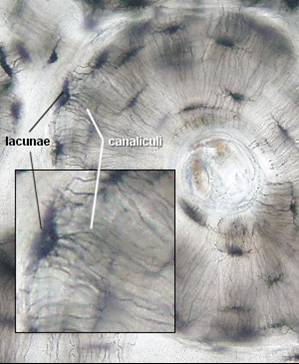
\includegraphics[width=0.14\linewidth]
      {\figDirHomBones//cortical-bone}
      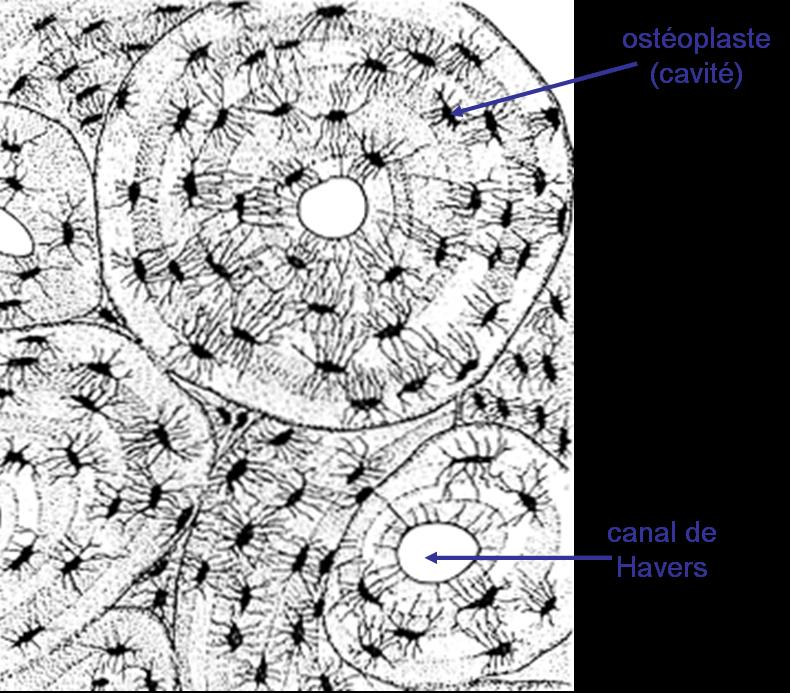
\includegraphics[width=0.2\linewidth]
      {\figDirHomBones//cortical-bone-sketch}
    }
  \item given macroscopic deformation and pressure, recover
    \begin{itemize}
    \item displacements $\ub^{\mic}$, pressure $p^{\mic}$
    \item micro-level $\ell^{\mu_1}$, sub-micro-level $\ell^{\mu_2}$ diffusion
    \end{itemize}
  \end{itemize}
  \begin{center}
    \begin{minipage}{0.32\linewidth}
      \scriptsize
      micro: various topologies, corrector functions \\
      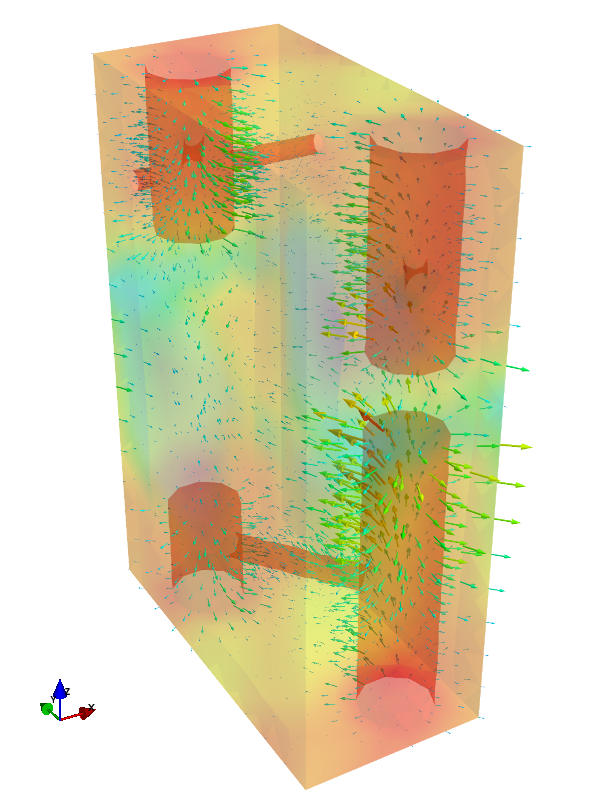
\includegraphics[width=0.48\linewidth]
      {\figDirHomBones/steady_rs_00_p_M1}
      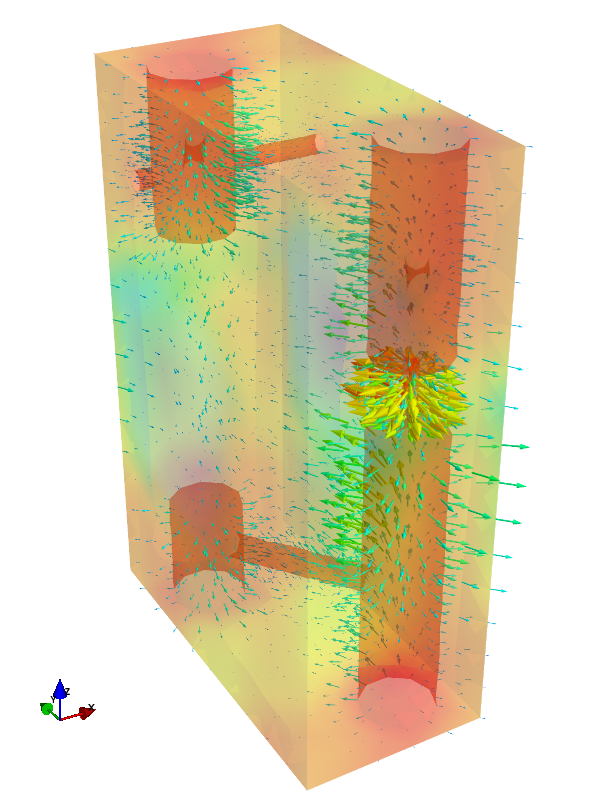
\includegraphics[width=0.48\linewidth]
      {\figDirHomBones/steady_rs_00_p_M2}
    \end{minipage}
    \hfill
    \begin{minipage}{0.17\linewidth}
      \scriptsize
      macro: compact bone segment \\
      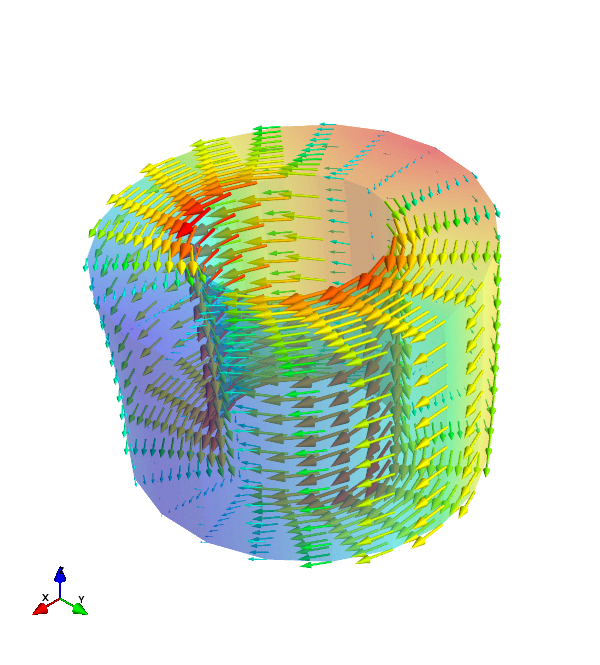
\includegraphics[width=0.9\linewidth]
      {\figDirHomBones/macro_t05_M2}
    \end{minipage}
    \hfill
    \begin{minipage}{0.45\linewidth}
      \scriptsize
      micro: recovery in a macro-point \\
      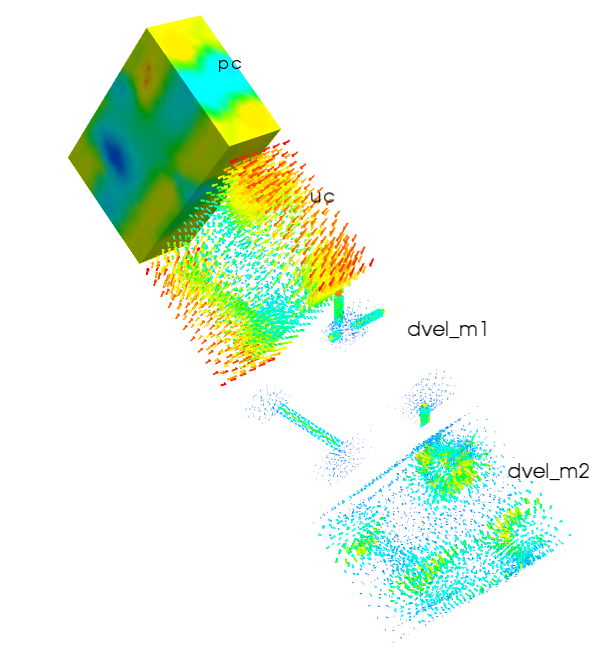
\includegraphics[width=0.48\linewidth]
      {\figDirHomBones/recovery_1999_200_M1}
      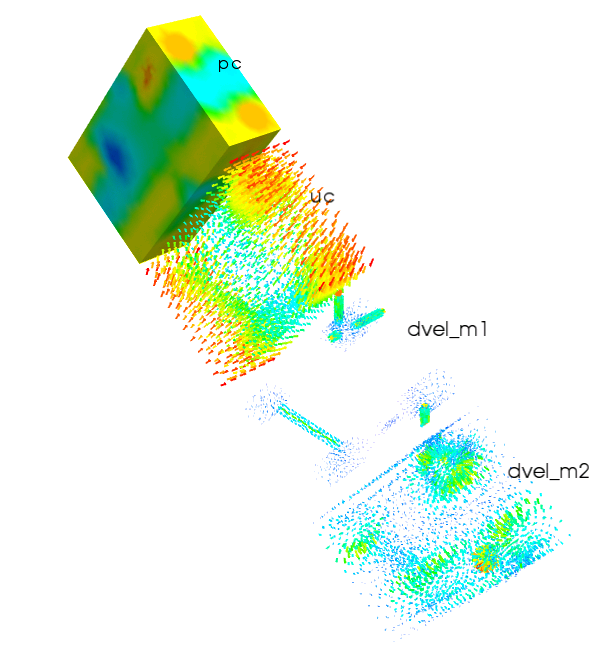
\includegraphics[width=0.48\linewidth]
      {\figDirHomBones/recovery_1999_200_M2}
    \end{minipage}
  \end{center}
\end{frame}
